\documentclass[10pt]{beamer}\usepackage[]{graphicx}\usepackage[]{color}
%% maxwidth is the original width if it is less than linewidth
%% otherwise use linewidth (to make sure the graphics do not exceed the margin)
\makeatletter
\def\maxwidth{ %
  \ifdim\Gin@nat@width>\linewidth
    \linewidth
  \else
    \Gin@nat@width
  \fi
}
\makeatother

\definecolor{fgcolor}{rgb}{0.345, 0.345, 0.345}
\newcommand{\hlnum}[1]{\textcolor[rgb]{0.686,0.059,0.569}{#1}}%
\newcommand{\hlstr}[1]{\textcolor[rgb]{0.192,0.494,0.8}{#1}}%
\newcommand{\hlcom}[1]{\textcolor[rgb]{0.678,0.584,0.686}{\textit{#1}}}%
\newcommand{\hlopt}[1]{\textcolor[rgb]{0,0,0}{#1}}%
\newcommand{\hlstd}[1]{\textcolor[rgb]{0.345,0.345,0.345}{#1}}%
\newcommand{\hlkwa}[1]{\textcolor[rgb]{0.161,0.373,0.58}{\textbf{#1}}}%
\newcommand{\hlkwb}[1]{\textcolor[rgb]{0.69,0.353,0.396}{#1}}%
\newcommand{\hlkwc}[1]{\textcolor[rgb]{0.333,0.667,0.333}{#1}}%
\newcommand{\hlkwd}[1]{\textcolor[rgb]{0.737,0.353,0.396}{\textbf{#1}}}%
\let\hlipl\hlkwb

\usepackage{framed}
\makeatletter
\newenvironment{kframe}{%
 \def\at@end@of@kframe{}%
 \ifinner\ifhmode%
  \def\at@end@of@kframe{\end{minipage}}%
  \begin{minipage}{\columnwidth}%
 \fi\fi%
 \def\FrameCommand##1{\hskip\@totalleftmargin \hskip-\fboxsep
 \colorbox{shadecolor}{##1}\hskip-\fboxsep
     % There is no \\@totalrightmargin, so:
     \hskip-\linewidth \hskip-\@totalleftmargin \hskip\columnwidth}%
 \MakeFramed {\advance\hsize-\width
   \@totalleftmargin\z@ \linewidth\hsize
   \@setminipage}}%
 {\par\unskip\endMakeFramed%
 \at@end@of@kframe}
\makeatother

\definecolor{shadecolor}{rgb}{.97, .97, .97}
\definecolor{messagecolor}{rgb}{0, 0, 0}
\definecolor{warningcolor}{rgb}{1, 0, 1}
\definecolor{errorcolor}{rgb}{1, 0, 0}
\newenvironment{knitrout}{}{} % an empty environment to be redefined in TeX

\usepackage{alltt}

%% include header:
\usetheme{metropolis}
\usepackage{appendixnumberbeamer}

\usepackage{booktabs}
\usepackage[scale=2]{ccicons}

\usepackage{pgfplots}
\usepgfplotslibrary{dateplot}

\usepackage{xspace}
\newcommand{\themename}{\textbf{\textsc{metropolis}}\xspace}

\usepackage[english]{babel}
\usepackage{dsfont}
\usepackage{amsmath}
\usepackage{amssymb}
\usepackage{amsthm}
\usepackage{amsfonts}
\usepackage[utf8]{inputenc}

%% Define theme color(s):
%% ---------------------------------------------------------------

\usepackage{xcolor}

% \definecolor{metropolis_theme_color}{RGB}{35,55,59}
\definecolor{metropolis_theme_color}{RGB}{42,42,42}

%% Color custimzations:
\definecolor{blue}{RGB}{0,155,164}
\definecolor{lime}{RGB}{175,202,11}
\definecolor{green}{RGB}{0,137,62}
\definecolor{titleblue}{RGB}{4,58,63}
\definecolor{deepskyblue}{RGB}{0,191,255}
\definecolor{mygrey}{RGB}{240,240,240}

\setbeamercolor{frametitle}{fg=mygrey, bg=metropolis_theme_color}
\setbeamercolor{progress bar}{fg=metropolis_theme_color}

%% Shaded for nicer code highlighting:
%% ---------------------------------------------------------------

\usepackage{mdframed}
% \usepackage{verbatim}

% Define Shaded if not defined:
\makeatletter
\@ifundefined{Shaded}{%
  \newenvironment{Shaded}{\begin{snugshade}}{\end{snugshade}}%
}{}
\makeatother

\renewenvironment{Shaded}{
  \begin{mdframed}[
    backgroundcolor=mygrey,
    linecolor=metropolis_theme_color,
    rightline=false,
		leftline=false
  ]}{
  \end{mdframed}
}

%% Title Image:
%% ---------------------------------------------------------------

% Load transparent:
\usepackage{transparent}

% Add titlegraphic:
\titlegraphic{
  \vspace{2cm}
  \hspace{5.03cm}
  \transparent{0.2}
  
\includegraphics[width=8cm]{images/logos/LMU}
}

%% Adjust frame number to be displayd as i/n:
%% ---------------------------------------------------------------
\setbeamertemplate{frame numbering}{%
  \insertframenumber{}/\inserttotalframenumber
}
\makeatother


%% Include latex-math:
%% ---------------------------------------------------------------
% Include latex-math
\DeclareOldFontCommand{\sf}{\normalfont\sffamily}{\mathsf}

\IfFileExists{./latex-math/basic-math.tex}{
  \input{./latex-math/basic-math.tex}
  \input{./latex-math/ml-bagging.tex}
  \input{./latex-math/ml-boosting.tex}
  \input{./latex-math/ml-gp.tex}
  \input{./latex-math/ml-mbo.tex}
  \input{./latex-math/ml-nn.tex}
  \input{./latex-math/ml-svm.tex}
  \input{./latex-math/ml-trees.tex}
}{
  \IfFileExists{./../latex-math/basic-math.tex}{
    \input{./../latex-math/basic-math.tex}
    \input{./../latex-math/basic-ml.tex}
    \input{./../latex-math/ml-bagging.tex}
    \input{./../latex-math/ml-boosting.tex}
    \input{./../latex-math/ml-gp.tex}
    \input{./../latex-math/ml-mbo.tex}
    \input{./../latex-math/ml-nn.tex}
    \input{./../latex-math/ml-svm.tex}
    \input{./../latex-math/ml-trees.tex}
  }{}
}

%% Style URLs
%% ---------------------------------------------------------------

\usepackage{hyperref}

\definecolor{myorange}{RGB}{225, 127, 0}
\renewcommand\UrlFont{\color{myorange}}


%% include template:
%% Footer:
\usepackage{xfrac}
\usepackage{framed, color}

\setbeamertemplate{footline}[text line]{%
    \noindent\hspace*{\dimexpr-\oddsidemargin-1in\relax}%
     \colorbox{metropolis_theme_color}{
     \makebox[\dimexpr\paperwidth-2\fboxsep\relax]{
     \color{mygrey}
     \begin{minipage}{0.33\linewidth}
       \secname
     \end{minipage}\hfill
     \begin{minipage}{0.33\linewidth}
       \centering
       \insertshortauthor
     \end{minipage}\hfill
     \begin{minipage}{0.33\linewidth}
       \flushright
       \insertframenumber{}/\inserttotalframenumber
     \end{minipage}     
     }}%
  \hspace*{-\paperwidth}
}



%% kableExtra stuff:
%% ----------------------------------------

\usepackage{booktabs}
\usepackage{longtable}
\usepackage{array}
\usepackage{multirow}
\usepackage{wrapfig}
\usepackage{float}
\usepackage{colortbl}
\usepackage{pdflscape}
\usepackage{tabu}
\usepackage{threeparttable}
\usepackage{threeparttablex}
\usepackage[normalem]{ulem}
\usepackage{makecell}
\usepackage{xcolor}


\definecolor{metropolis_orange}{RGB}{225, 127, 0}


%% Title:
%% ----------------------------------------

\title{compboost}
\subtitle{Fast and Flexible Component-Wise Boosting Framework}
% \date{\today}
\date{July 12, 2019}
\author{\textbf{Daniel Schalk}, Janek Thomas, and Bernd Bischl}
\institute{LMU Munich\\Working Group Computational Statistics}

%% Wrap Shaded around Shunk to have a nices R output:
%% --------------------------------------------------

\let\Oldkframe\kframe
\let\endOldkframe\endkframe

\renewenvironment{kframe}
 {\scriptsize\definecolor{shadecolor}{RGB}{240,240,240}\begin{Shaded}\Oldkframe}
 {\endOldkframe\end{Shaded}\normalsize}

%% Prevent code from printing over margin:
%% --------------------------------------------------



%% Content:
%% ----------------------------------------
\IfFileExists{upquote.sty}{\usepackage{upquote}}{}
\begin{document}







%% SETUP Chunk:
%% ----------------------------------------



\maketitle



\section{Use-Case}

\begin{frame}{The Situation}

\begin{itemize}
  \item
    We own a small booth at the city center that sells beer.

  \item
    As we are very interested in our customers' health, we only sell to customers who we expect to drink less than 110 liters per year.

  \item
    To estimate how much a customer drinks, we have collected data from 200 customers in recent years.

  \item
    These data include the beer consumption (in liter), age, sex, country of origin, weight, body size, and 200 characteristics gained from app usage (that have absolutely no influence).
\end{itemize}

\end{frame}

\begin{frame}[fragile]{Overview of the Data}

\begin{knitrout}
\definecolor{shadecolor}{rgb}{0.969, 0.969, 0.969}\color{fgcolor}\begin{table}[H]
\centering
\resizebox{\linewidth}{!}{
\begin{tabular}{rllrrrrlr}
\toprule
\textbf{beer\_consumption} & \textbf{gender} & \textbf{country} & \textbf{age} & \textbf{weight} & \textbf{height} & \textbf{app\_usage1} & \textbf{...} & \textbf{app\_usage200}\\
\midrule
\rowcolor{gray!6}  106.5 & m & Seychelles & 33 & 87.17 & 172.9 & 0.1680 & ... & 0.1313\\
85.5 & f & Seychelles & 52 & 89.38 & 200.4 & 0.8075 & ... & 0.6087\\
\rowcolor{gray!6}  116.5 & f & Czechia & 54 & 92.03 & 178.7 & 0.3849 & ... & 0.5786\\
67.0 & m & Australia & 32 & 63.53 & 186.3 & 0.3277 & ... & 0.3594\\
\rowcolor{gray!6}  43.0 & f & Australia & 51 & 64.73 & 175.0 & 0.6021 & ... & 0.7406\\
\addlinespace
85.0 & m & Austria & 43 & 95.74 & 173.2 & 0.6044 & ... & 0.4181\\
\rowcolor{gray!6}  79.0 & f & Austria & 55 & 87.65 & 156.3 & 0.1246 & ... & 0.4398\\
107.0 & f & Austria & 24 & 93.17 & 161.4 & 0.2946 & ... & 0.6130\\
\rowcolor{gray!6}  57.0 & m & USA & 55 & 76.27 & 182.5 & 0.5776 & ... & 0.4927\\
89.0 & m & USA & 16 & 72.21 & 203.3 & 0.6310 & ... & 0.0735\\
\bottomrule
\end{tabular}}
\end{table}


\end{knitrout}

\end{frame}


\begin{frame}{Our Goals}

With these data we want to answer the following questions:

\begin{itemize}
  \item
    Which of the customers' characteristics are important to be able to determine the consumption?
  \item
    How does the effect of important features look like?
  \item
    How does the model behave on unseen data?
\end{itemize}

\end{frame}




\section{What is Component-Wise Boosting?}

\begin{frame}{General Idea}

\begin{center}
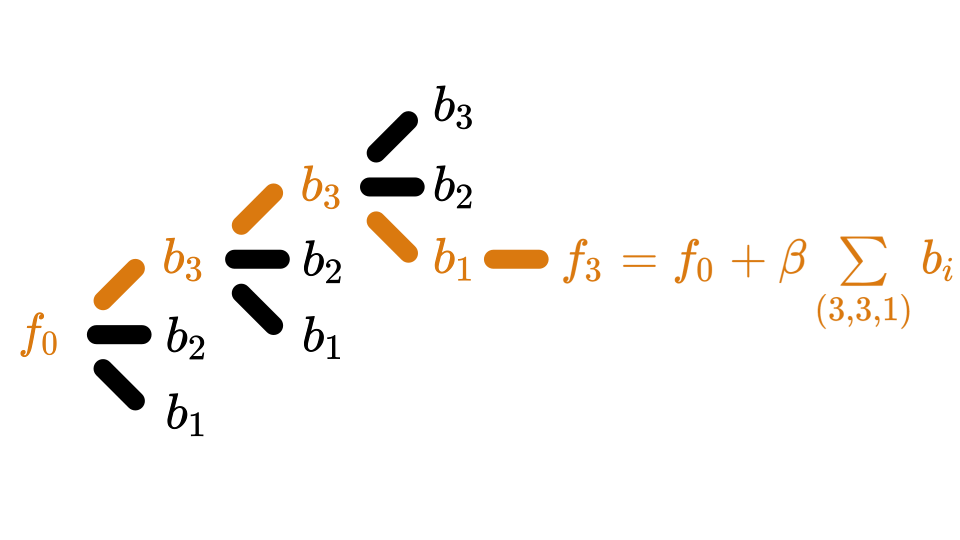
\includegraphics[width=0.8\textwidth]{./images/cboost_gif_norisk.png}
\end{center}

\vspace{-1cm}

\begin{itemize}

  \item
    Sequential fitting of the base-learner $b_1, b_2, b_3$ on the error / pseudo-residuals of the current ensemble.

  \item
    The base-learner with the best fit on the error (measured as mean squared error) is added to the ensemble.

  \item
    Results in a weighted sum / additive model over base-learners.

\end{itemize}

\end{frame}

\begin{frame}{Advantages of Component-Wise Boosting}

  \begin{itemize}

    \item
      Inherent (unbiased) feature selection.

    \item
      Resulting model is sparse since important effects are selected first and therefore it is able to learn in high-dimensional feature spaces ($p \gg n$).

    \item
      Parameters are updated iteratively. Therefore, the whole trace of how the model evolves is available. \vspace{0.3cm}



\begin{knitrout}
\definecolor{shadecolor}{rgb}{0.969, 0.969, 0.969}\color{fgcolor}

{\centering 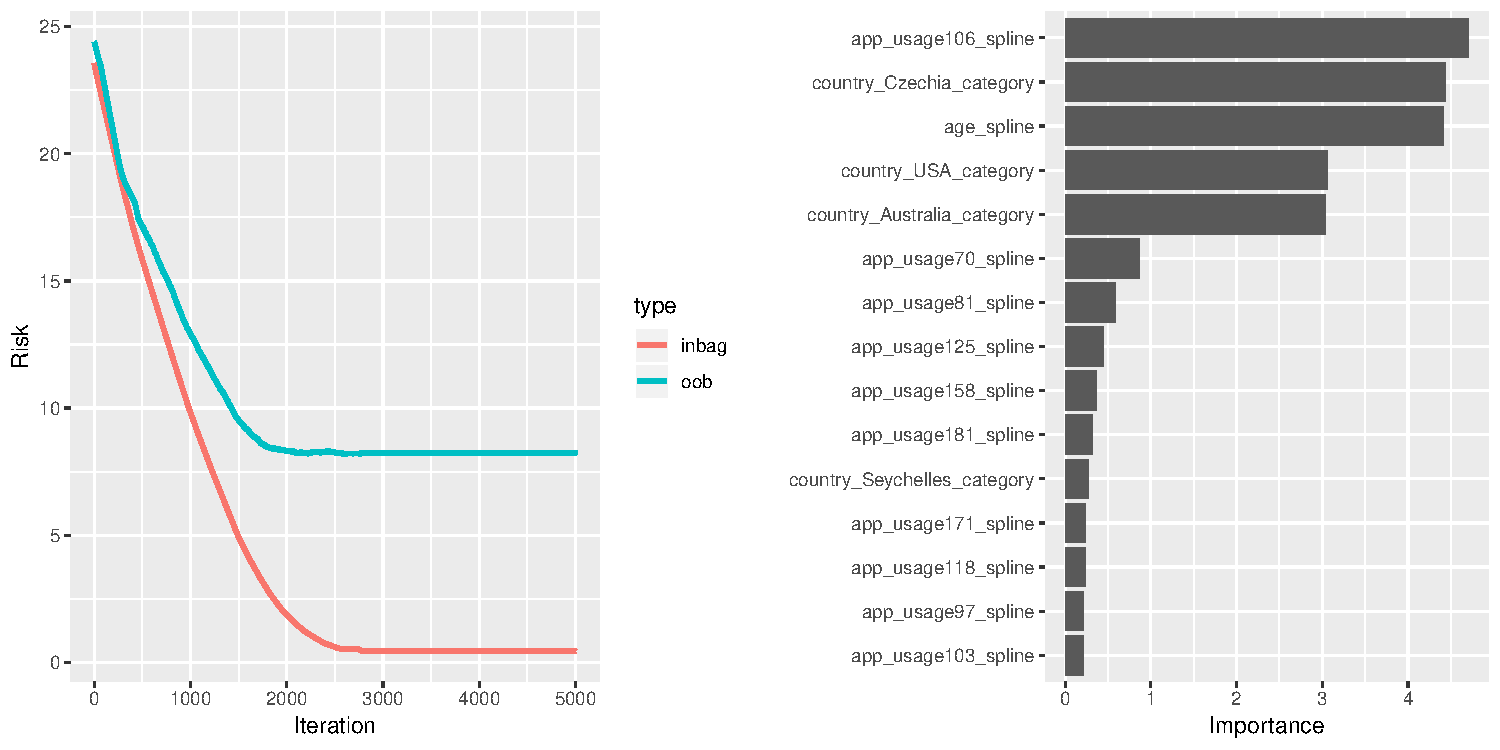
\includegraphics[width=0.7\textwidth]{figure/unnamed-chunk-5-1} 

}



\end{knitrout}



  \end{itemize}

\end{frame}




\section{About Compboost}

\begin{frame}{Current Standard}

Most popular package for model-based boosting is \texttt{mboost}:

\begin{itemize}

  \item
    Large number of available base-learner and losses.

  \item
    Extended to more complex problems:
    \begin{itemize}
      \item Functional data
      \item GAMLSS models
      \item Survival analysis
    \end{itemize}
  \item
    Extendible with custom base-learner and losses.

\end{itemize}

\textbf{So, why another boosting implementation?}

\begin{itemize}

  \item
    Main parts of \texttt{mboost} are written in \texttt{R} and gets slow for large datasets.

  \item
    Complex implementation:
    \begin{itemize}
      \item Nested scopes
      \item Mixture of different \texttt{R} class systems
    \end{itemize}
\end{itemize}

\end{frame}


\begin{frame}{About Compboost}


Fast and flexible framework for model-based boosting:

\begin{itemize}

  \item
    With \texttt{mboost} as standard, we want to keep the modular principle of defining custom base-learner and losses.

  \item
    Completely written in \texttt{C++} and exposed by \texttt{Rcpp} to obtain high performance and full memory control.

  \item
    \texttt{R} API is written in \texttt{R6} to provide convenient wrapper.

  \item
    Major parts of the \texttt{compboost} functionality are unit tested against \texttt{mboost} to ensure correctness.

\end{itemize}

\end{frame}



\section{Small Demonstration}

\begin{frame}[fragile]{Starting With Convenience Wrapper}

\texttt{boostLinear()} and \texttt{boostSplines()} automatically adds univariate linear models or a GAM for all features.

\begin{knitrout}
\definecolor{shadecolor}{rgb}{0.969, 0.969, 0.969}\color{fgcolor}\begin{kframe}
\begin{alltt}
\hlkwd{set.seed}\hlstd{(}\hlnum{618}\hlstd{)}
\hlstd{cboost} \hlkwb{=} \hlkwd{boostSplines}\hlstd{(}\hlkwc{data} \hlstd{= beer_data,} \hlkwc{target} \hlstd{=} \hlstr{"beer_consumption"}\hlstd{,}
  \hlkwc{loss} \hlstd{= LossAbsolute}\hlopt{$}\hlkwd{new}\hlstd{(),} \hlkwc{learning_rate} \hlstd{=} \hlnum{0.1}\hlstd{,} \hlkwc{iterations} \hlstd{=} \hlnum{5000L}\hlstd{,}
  \hlkwc{penalty} \hlstd{=} \hlnum{10}\hlstd{,} \hlkwc{oob_fraction} \hlstd{=} \hlnum{0.3}\hlstd{,} \hlkwc{trace} \hlstd{=} \hlnum{2500L}\hlstd{)}
\end{alltt}
\begin{verbatim}
##    1/5000   risk = 24  oob_risk = 24   
## 2500/5000   risk = 0.6  oob_risk = 8.3   
## 5000/5000   risk = 0.44  oob_risk = 8.3   
## 
## 
## Train 5000 iterations in 12 Seconds.
## Final risk based on the train set: 0.44
\end{verbatim}
\end{kframe}
\end{knitrout}

\end{frame}

\begin{frame}[fragile]{Visualizing the Results}

\begin{knitrout}
\definecolor{shadecolor}{rgb}{0.969, 0.969, 0.969}\color{fgcolor}\begin{kframe}
\begin{alltt}
\hlstd{gg1} \hlkwb{=} \hlstd{cboost}\hlopt{$}\hlkwd{plotInbagVsOobRisk}\hlstd{()}
\hlstd{gg2} \hlkwb{=} \hlstd{cboost}\hlopt{$}\hlkwd{plotFeatureImportance}\hlstd{()}
\end{alltt}
\end{kframe}
\end{knitrout}

\begin{knitrout}
\definecolor{shadecolor}{rgb}{0.969, 0.969, 0.969}\color{fgcolor}
\includegraphics[width=\textwidth]{figure/unnamed-chunk-8-1} 

\end{knitrout}

\end{frame}

\begin{frame}[fragile]{Visualizing the Results}

\begin{knitrout}
\definecolor{shadecolor}{rgb}{0.969, 0.969, 0.969}\color{fgcolor}\begin{kframe}
\begin{alltt}
\hlstd{cboost}\hlopt{$}\hlkwd{train}\hlstd{(}\hlnum{2000L}\hlstd{)}

\hlstd{gg1} \hlkwb{=} \hlstd{cboost}\hlopt{$}\hlkwd{plotFeatureImportance}\hlstd{()}
\hlstd{gg2} \hlkwb{=} \hlstd{cboost}\hlopt{$}\hlkwd{plot}\hlstd{(}\hlstr{"age_spline"}\hlstd{,} \hlkwc{iters} \hlstd{=} \hlkwd{c}\hlstd{(}\hlnum{50}\hlstd{,} \hlnum{100}\hlstd{,} \hlnum{500}\hlstd{,} \hlnum{1000}\hlstd{,} \hlnum{2000}\hlstd{,} \hlnum{4000}\hlstd{))}
\end{alltt}
\end{kframe}
\end{knitrout}


\begin{knitrout}
\definecolor{shadecolor}{rgb}{0.969, 0.969, 0.969}\color{fgcolor}
\includegraphics[width=\textwidth]{figure/unnamed-chunk-10-1} 

\end{knitrout}

\end{frame}

\begin{frame}[fragile]{Using the R6 Interface}

\begin{knitrout}
\definecolor{shadecolor}{rgb}{0.969, 0.969, 0.969}\color{fgcolor}\begin{kframe}
\begin{alltt}
\hlstd{cboost} \hlkwb{=} \hlstd{Compboost}\hlopt{$}\hlkwd{new}\hlstd{(}\hlkwc{data} \hlstd{= beer_data,} \hlkwc{target} \hlstd{=} \hlstr{"beer_consumption"}\hlstd{,}
  \hlkwc{loss} \hlstd{= LossQuantile}\hlopt{$}\hlkwd{new}\hlstd{(}\hlnum{0.9}\hlstd{),} \hlkwc{learning_rate} \hlstd{=} \hlnum{0.1}\hlstd{,} \hlkwc{oob_fraction} \hlstd{=} \hlnum{0.3}\hlstd{)}

\hlstd{cboost}\hlopt{$}\hlkwd{addBaselearner}\hlstd{(}\hlstr{"age"}\hlstd{,} \hlstr{"spline"}\hlstd{, BaselearnerPSpline)}
\hlstd{cboost}\hlopt{$}\hlkwd{addBaselearner}\hlstd{(}\hlstr{"country"}\hlstd{,} \hlstr{"category"}\hlstd{, BaselearnerPolynomial)}

\hlstd{cboost}\hlopt{$}\hlkwd{addLogger}\hlstd{(}\hlkwc{logger} \hlstd{= LoggerTime,} \hlkwc{use_as_stopper} \hlstd{=} \hlnum{TRUE}\hlstd{,} \hlkwc{logger_id} \hlstd{=} \hlstr{"time"}\hlstd{,}
  \hlkwc{max_time} \hlstd{=} \hlnum{2e5}\hlstd{,} \hlkwc{time_unit} \hlstd{=} \hlstr{"microseconds"}\hlstd{)}

\hlstd{cboost}\hlopt{$}\hlkwd{train}\hlstd{(}\hlnum{10000}\hlstd{,} \hlkwc{trace} \hlstd{=} \hlnum{500}\hlstd{)}
\end{alltt}
\begin{verbatim}
##     1/10000   risk = 11  oob_risk = 10   time = 0   
##   500/10000   risk = 7.9  oob_risk = 8.2   time = 20162   
##  1000/10000   risk = 6.3  oob_risk = 6.6   time = 43488   
##  1500/10000   risk = 5.1  oob_risk = 5.4   time = 73143   
##  2000/10000   risk = 4.2  oob_risk = 4.5   time = 117189   
##  2500/10000   risk = 3.5  oob_risk = 3.8   time = 160851   
## 
## 
## Train 2905 iterations in 0 Seconds.
## Final risk based on the train set: 3.2
\end{verbatim}
\end{kframe}
\end{knitrout}

\end{frame}

\begin{frame}{Overview of the Functionality}

\begin{itemize}

  \item
    \textbf{Base-learner:} \texttt{BaselearnerPolynomial}, \texttt{BaselearnerSpline}, \texttt{BaselearnerCustom}, and \texttt{BaselearnerCustomCpp}

  \item
    \textbf{Loss functions:} \texttt{LossQuadratic}, \texttt{LossAbsolute}, \texttt{LossQuantile}, \texttt{LossHuber}, \texttt{LossBinomial}, \texttt{LossCustom}, and \texttt{LossCustomCpp}

  \item
    \textbf{Logger/Stopper:} \texttt{LoggerIteration}, \texttt{LoggerInbagRisk}, \texttt{LoggerOobRisk}, and \texttt{LoggerTime} \\
    \begin{itemize}
      \item[$\rightarrow$]
        Performance-based early stopping can be applied using the \texttt{LoggerOobRisk} and specifying the relative improvement that should be reached (e.g. 0 for stopping when out of bag risk starts to increase).
    \end{itemize}

\end{itemize}

\end{frame}

\section{Performance Considerations}

\begin{frame}{Performance Considerations}


\begin{itemize}

  \item
    Optimizer are parallelized via openmp:\vspace{0.3cm}

\begin{knitrout}
\definecolor{shadecolor}{rgb}{0.969, 0.969, 0.969}\color{fgcolor}

{\centering \includegraphics[width=0.7\textwidth]{figure/unnamed-chunk-12-1} 

}



\end{knitrout}

  \item
    Take advantage of the matrix structure to speed up the algorithm by reducing the number of repetitive or too expensive calculations.

  \item
    Matrices are stored (if possible) as a sparse matrix.

\end{itemize}

\end{frame}

\begin{frame}{Small Comparison With Mboost}

\begin{itemize}

  \item
    Runtime (in minutes):\vspace{-0.3cm}
    \begin{table}[H]
    \centering
    \resizebox{\linewidth}{!}{
      \begin{tabular}{c|c|c|c}
        \textbf{nrows / ncols} & \parbox{3cm}{\centering \textbf{mboost}} & \parbox{3cm}{\centering \textbf{compboost}} & \parbox{3cm}{\centering \textbf{compboost} \\ \textbf{(16 threads)}} \\
        \midrule
        20000 / 200  &  21.10 (1) &  10.47 (2.02) & 0.95 (22.21) \\
        20000 / 2000 & 216.70 (1) &  83.95 (2.58) & 8.15 (26.59)
      \end{tabular}
    }
    \end{table}

  \item
    Memory (in GB):\vspace{-0.3cm}
    \begin{table}[H]
    \centering
    \resizebox{\linewidth}{!}{
      \begin{tabular}{c|c|c|c}
        \textbf{nrows / ncols} & \parbox{3cm}{\centering \textbf{mboost}} & \parbox{3cm}{\centering \textbf{compboost}} & \parbox{3cm}{\centering \textbf{compboost} \\ \textbf{(16 threads)}} \\
        \midrule
        20000 / 200  & 1.04 (1) & 0.28 (3.71) & 0.30 (3.47) \\
        20000 / 2000 & 8.70 (1) & 2.60 (3.35) & 2.98 (2.92)
      \end{tabular}
    }
    \end{table}

\end{itemize}

(Comparison was made by just using spline base-learner with 20 knots and and 5000 iterations. The numbers in the brackets are the relative values compared to \texttt{mboost}.)


% \begin{table}[H]
% \centering
% \resizebox{\linewidth}{!}{
% \begin{tabular}{c||c|c||c|c||c|c}
%  & \multicolumn{2}{c||}{\textbf{mboost}} & \multicolumn{2}{c||}{\textbf{compboost}} & \multicolumn{2}{c}{\textbf{compboost (16 threads)}} \\
%  \textbf{nrows / ncols} & \textbf{Memory Usage} & \textbf{Runtime} & \textbf{Memory Usage} & \textbf{Runtime} & \textbf{Memory Usage} & \textbf{Runtime} \\
% \midrule
% 20000 / 200  & 1.04 (1) &  21.1 (1) & 0.28 (3.7) & 10.47 (2) & 0.3 (3.5)  & 0.95 (22) \\
% 20000 / 2000 & 8.70 (1) & 216.7 (1) & 2.60 (3.3) & 83.95 (2.5) & 2.98 (3) & 8.15 (25)
% \end{tabular}
% }
% \end{table}

\end{frame}


\section{What's Next?}

\begin{frame}{What's Next?}

\begin{itemize}
  \item
    Research on computational aspects of the algorithm:
    \begin{itemize}
      \item
        More stable base-learner selection process via resampling
      \item
        Base-learner selection for arbitrary performance measures
      \item
        Smarter and faster optimizers
    \end{itemize}

  \item
    Greater functionality:
    \begin{itemize}
      \item
        Functional data structures and loss functions
      \item
        Unbiased feature selection
      \item
        Effect decomposition into constant, linear, and non-linear
    \end{itemize}

    \item
      Reducing the memory load by applying binning on numerical features.

    \item
      Adding hyperparameter tuning by providing a \texttt{mlr} (\texttt{mlr3}) learner API.

    \item
      Exposing \texttt{C++} classes to python.
\end{itemize}

\end{frame}

% \addtocounter{framenumber}{-1}

\begin{frame}

\begin{itemize}

  \item
    Slides are available at:
    \vspace{0.2cm}
    \begin{center}
      \url{www.github.com/schalkdaniel/compboost_talk_useR}
    \end{center}
    \vspace{0.3cm}

  \item
    Actively developed on GitHub:
    \vspace{0.2cm}
    \begin{center}
      \url{www.github.com/schalkdaniel/compboost}
    \end{center}
    \vspace{0.3cm}

  \item
    Project page:
    \vspace{0.2cm}
    \begin{center}
      \url{www.compboost.org}
    \end{center}
    \vspace{0.3cm}

  \item
    JOSS DOI:
    \vspace{0.2cm}
    \begin{center}
      \href{https://joss.theoj.org/papers/94cfdbbfdfc8796c5bdb1a74ee59fcda}{\textcolor{metropolis_orange}{10.21105/joss.00967}}
    \end{center}

\end{itemize}

\end{frame}


\end{document}
